\documentclass[]{book}
\usepackage{lmodern}
\usepackage{amssymb,amsmath}
\usepackage{ifxetex,ifluatex}
\usepackage{fixltx2e} % provides \textsubscript
\ifnum 0\ifxetex 1\fi\ifluatex 1\fi=0 % if pdftex
  \usepackage[T1]{fontenc}
  \usepackage[utf8]{inputenc}
\else % if luatex or xelatex
  \ifxetex
    \usepackage{mathspec}
  \else
    \usepackage{fontspec}
  \fi
  \defaultfontfeatures{Ligatures=TeX,Scale=MatchLowercase}
\fi
% use upquote if available, for straight quotes in verbatim environments
\IfFileExists{upquote.sty}{\usepackage{upquote}}{}
% use microtype if available
\IfFileExists{microtype.sty}{%
\usepackage{microtype}
\UseMicrotypeSet[protrusion]{basicmath} % disable protrusion for tt fonts
}{}
\usepackage[margin=1in]{geometry}
\usepackage{hyperref}
\hypersetup{unicode=true,
            pdftitle={Internet of Things for Smart Industry},
            pdfauthor={Franz Maurer, Witek ten Hove \& Deny Smeets},
            pdfborder={0 0 0},
            breaklinks=true}
\urlstyle{same}  % don't use monospace font for urls
\usepackage{natbib}
\bibliographystyle{apalike}
\usepackage{longtable,booktabs}
\usepackage{graphicx,grffile}
\makeatletter
\def\maxwidth{\ifdim\Gin@nat@width>\linewidth\linewidth\else\Gin@nat@width\fi}
\def\maxheight{\ifdim\Gin@nat@height>\textheight\textheight\else\Gin@nat@height\fi}
\makeatother
% Scale images if necessary, so that they will not overflow the page
% margins by default, and it is still possible to overwrite the defaults
% using explicit options in \includegraphics[width, height, ...]{}
\setkeys{Gin}{width=\maxwidth,height=\maxheight,keepaspectratio}
\IfFileExists{parskip.sty}{%
\usepackage{parskip}
}{% else
\setlength{\parindent}{0pt}
\setlength{\parskip}{6pt plus 2pt minus 1pt}
}
\setlength{\emergencystretch}{3em}  % prevent overfull lines
\providecommand{\tightlist}{%
  \setlength{\itemsep}{0pt}\setlength{\parskip}{0pt}}
\setcounter{secnumdepth}{5}
% Redefines (sub)paragraphs to behave more like sections
\ifx\paragraph\undefined\else
\let\oldparagraph\paragraph
\renewcommand{\paragraph}[1]{\oldparagraph{#1}\mbox{}}
\fi
\ifx\subparagraph\undefined\else
\let\oldsubparagraph\subparagraph
\renewcommand{\subparagraph}[1]{\oldsubparagraph{#1}\mbox{}}
\fi

%%% Use protect on footnotes to avoid problems with footnotes in titles
\let\rmarkdownfootnote\footnote%
\def\footnote{\protect\rmarkdownfootnote}

%%% Change title format to be more compact
\usepackage{titling}

% Create subtitle command for use in maketitle
\newcommand{\subtitle}[1]{
  \posttitle{
    \begin{center}\large#1\end{center}
    }
}

\setlength{\droptitle}{-2em}
  \title{Internet of Things for Smart Industry}
  \pretitle{\vspace{\droptitle}\centering\huge}
  \posttitle{\par}
  \author{Franz Maurer, Witek ten Hove \& Deny Smeets}
  \preauthor{\centering\large\emph}
  \postauthor{\par}
  \predate{\centering\large\emph}
  \postdate{\par}
  \date{2017-06-05}

\usepackage{booktabs}
\usepackage{amsthm}
\makeatletter
\def\thm@space@setup{%
  \thm@preskip=8pt plus 2pt minus 4pt
  \thm@postskip=\thm@preskip
}
\makeatother

\usepackage{amsthm}
\newtheorem{theorem}{Theorem}[chapter]
\newtheorem{lemma}{Lemma}[chapter]
\theoremstyle{definition}
\newtheorem{definition}{Definition}[chapter]
\newtheorem{corollary}{Corollary}[chapter]
\newtheorem{proposition}{Proposition}[chapter]
\theoremstyle{definition}
\newtheorem{example}{Example}[chapter]
\theoremstyle{remark}
\newtheorem*{remark}{Remark}
\begin{document}
\maketitle

{
\setcounter{tocdepth}{1}
\tableofcontents
}
\chapter{- Welcome}\label{welcome}

This is an accompanying book to the HAN Minor Smart Industry and covers
the major topics regarding the Internet of Things (IoT) implementation
in an industrial setting.

\chapter{Introduction to IoT}\label{intro}

The IoT is the product of physical objects, controllers, sensors and
actuators and the internet \citep{mcewen_designing_2013}. The first
reference to the IoT was in 1982, when researchers at Carnegie Mellon
University developed the world's first IoT-enabled Coke Machine. Mark
Weiser developed the concept further in the early 90s; and Kevin Ashton
coined the term `Internet of Things' around 1999.

\chapter{IoT Capabilities}\label{capabilities}

 Your browser does not support this format.

\chapter{IoT Framework}\label{framework}

We describe our methods in this chapter.

\chapter{IoT Markets}\label{markets}

Some \emph{significant} applications are demonstrated in this chapter.

\section{Example one}\label{example-one}

\section{Example two}\label{example-two}

\chapter{IoT Fundamentals}\label{fundamentals}

We have finished a nice book.

\chapter{Sensors}\label{sensors}

We have finished a nice book.

\chapter{Data Communication}\label{communications}

We have finished a nice book.

\chapter{Cloud Platforms}\label{platforms}

We have finished a nice book.

\chapter{Privacy}\label{privacy}

We have finished a nice book.

\chapter{Security}\label{security}

We have finished a nice book.

\chapter{Encryption}\label{encryption}

We have finished a nice book.

\chapter{Data Analytics}\label{analytics}

\begin{figure}[htbp]
\centering
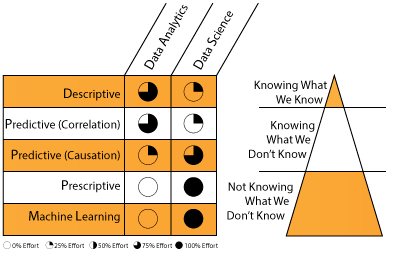
\includegraphics{./images/datascience.png}
\caption{Fig.12.1 - Data Analytics versus Science}
\end{figure}

\citep{j_data_2013}

\chapter{Dashboards and Apps}\label{apps}

We have finished a nice book.

\chapter{Arduino Programming}\label{arduino}

We have finished a nice book.

\bibliography{packages.bib,book.bib}


\end{document}
